\documentclass[11pt]{article}

\usepackage[margin=1in]{geometry}
\usepackage{amsmath, amssymb}
\usepackage{graphicx}
\usepackage{hyperref}

\title{A Numerical Study of \texttt{keccak256} Output Bits}
\author{Simon Tian}
\date{}

\begin{document}

\maketitle

\section{Introduction}

This note revises and completes the numerical study supporting the Gaussian
random number generator built from \texttt{keccak256}. The purpose of the study
is not to prove independence or exact fairness of the output bits, but to look
for empirical evidence against obvious failures of those assumptions over several
representative input families.

The conclusions should therefore be read as support for a practical modeling
choice, not as theorem-level validation. In particular, the study can show that
the tested diagnostics remain close to the values expected under a fair and
independent bit model, but it cannot prove full joint independence of the
256-bit output vector.

\section{Experiments}

Six experiment families are used:

\begin{enumerate}
\item sequential \texttt{uint256} values;
\item sequential \texttt{uint256} values shifted by $2^{128}$;
\item sequential strings of the form \texttt{Transaction Number: i};
\item shifted strings of the form \texttt{Transaction Number: }$2^{128}+i$;
\item random ASCII strings with length between $2$ and $7$;
\item random ASCII strings with length between $2$ and $32$.
\end{enumerate}

Each experiment contains $10{,}000$ hashes. For each experiment the study
records the bit-wise empirical means, pairwise similarity and correlation
metrics, input-bit correlations for sequential experiments, and autocorrelation
summaries up to lag $30$.

\section{Uniformity}

Figure~\ref{fig:uniformity} shows the estimated success probability of each bit
along with Bonferroni-adjusted confidence bands. Across all six experiments the
bit-wise estimates remain close to $0.5$, with no obvious structural drift by
bit position. In this run, the largest observed absolute deviation
$|\hat p_i - 0.5|$ lies between roughly $0.014$ and $0.019$ across the six
experiment families, which is small enough for the Gaussian paper's practical
normalization to remain plausible.

\begin{figure}[htbp]
\centering
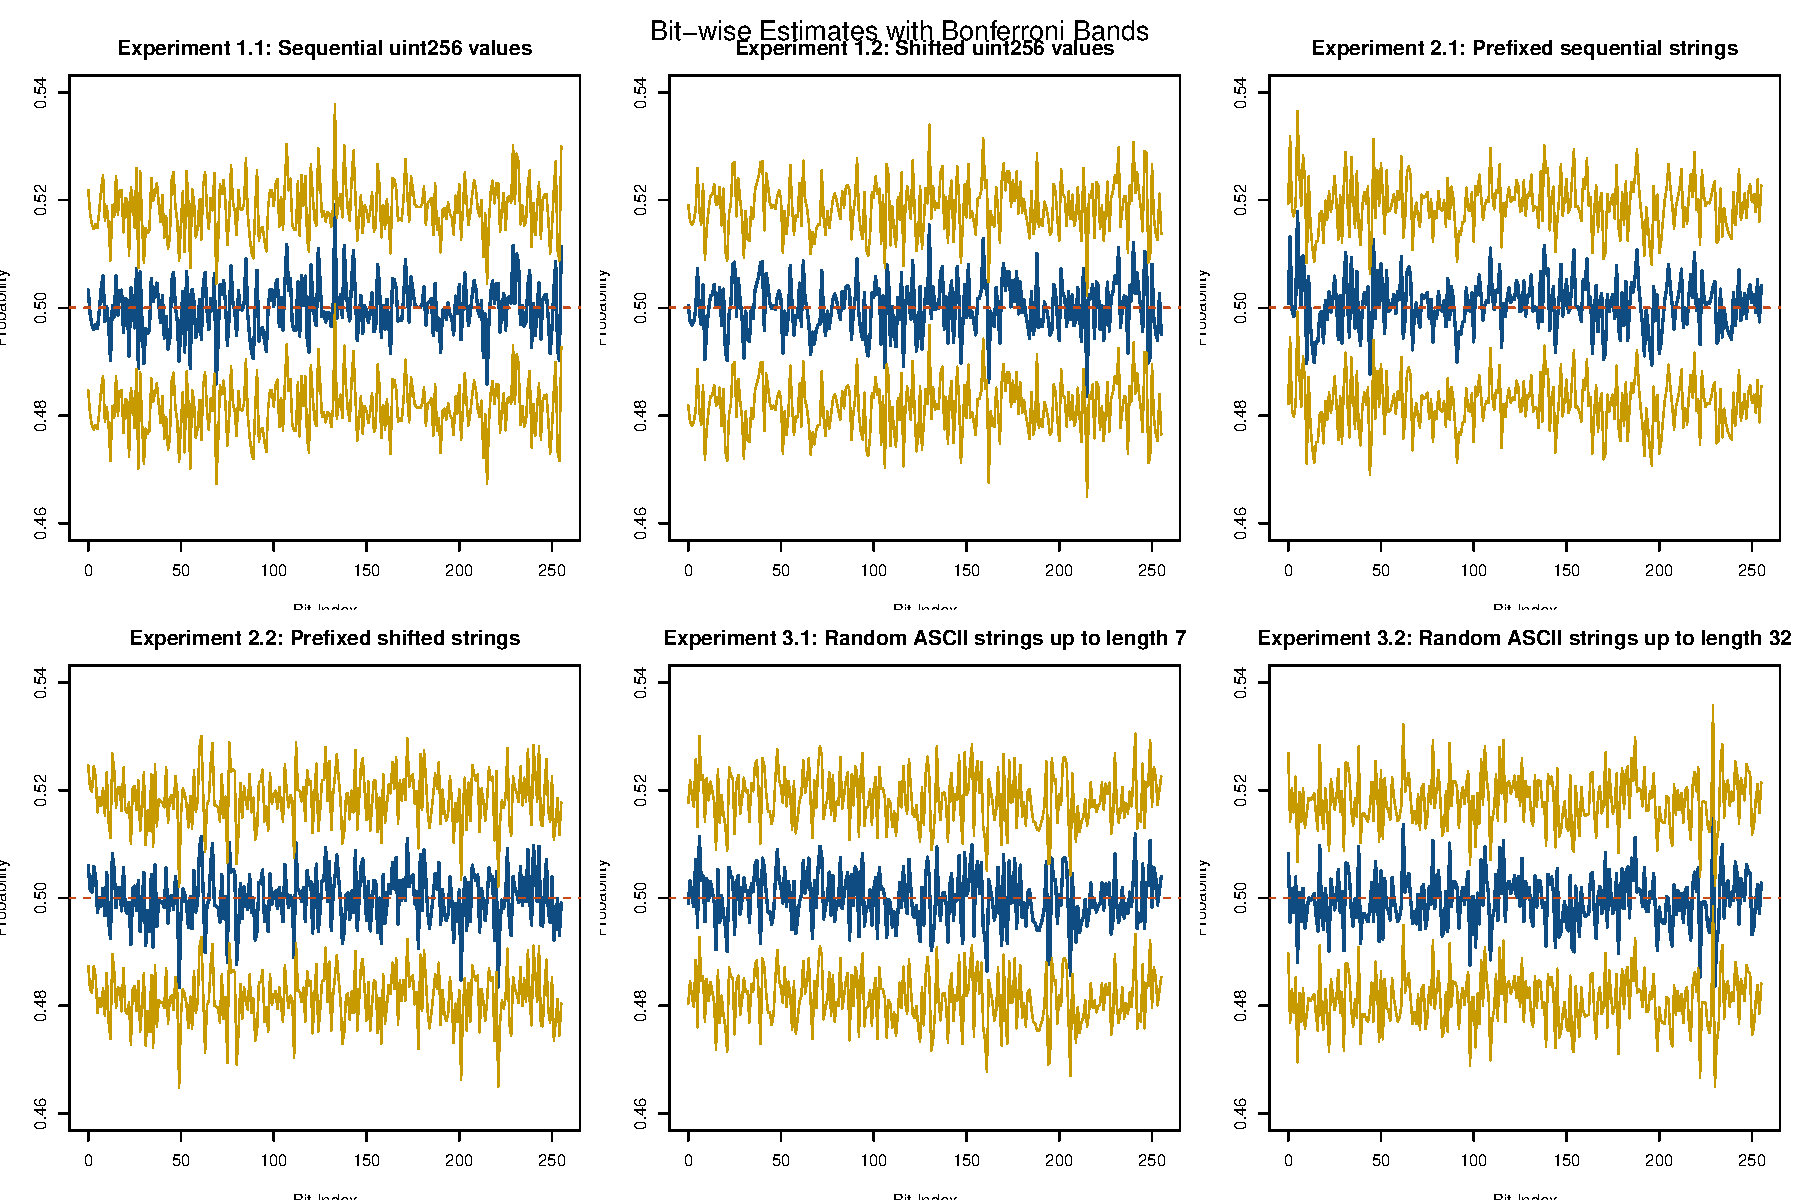
\includegraphics[width=\textwidth]{figures/uniformity_panels.pdf}
\caption{Bit-wise empirical means with Bonferroni-adjusted confidence bands for
all six experiment families.}
\label{fig:uniformity}
\end{figure}

\section{Dependence Diagnostics}

The first dependence diagnostic studies pairwise relationships among bits within
the baseline sequential integer experiment. Figure~\ref{fig:pairwise} shows the
distribution of Rogers-Tanimoto similarity, phi correlation, and
Sokal-Michener similarity over all $\binom{256}{2}$ bit pairs. The phi
correlation distribution is centered near zero, while the two similarity
measures remain concentrated near their fair-coin benchmarks. This is useful
evidence against simple pairwise dependence, but it should not be read as a
proof that higher-order dependence is absent.

\begin{figure}[htbp]
\centering
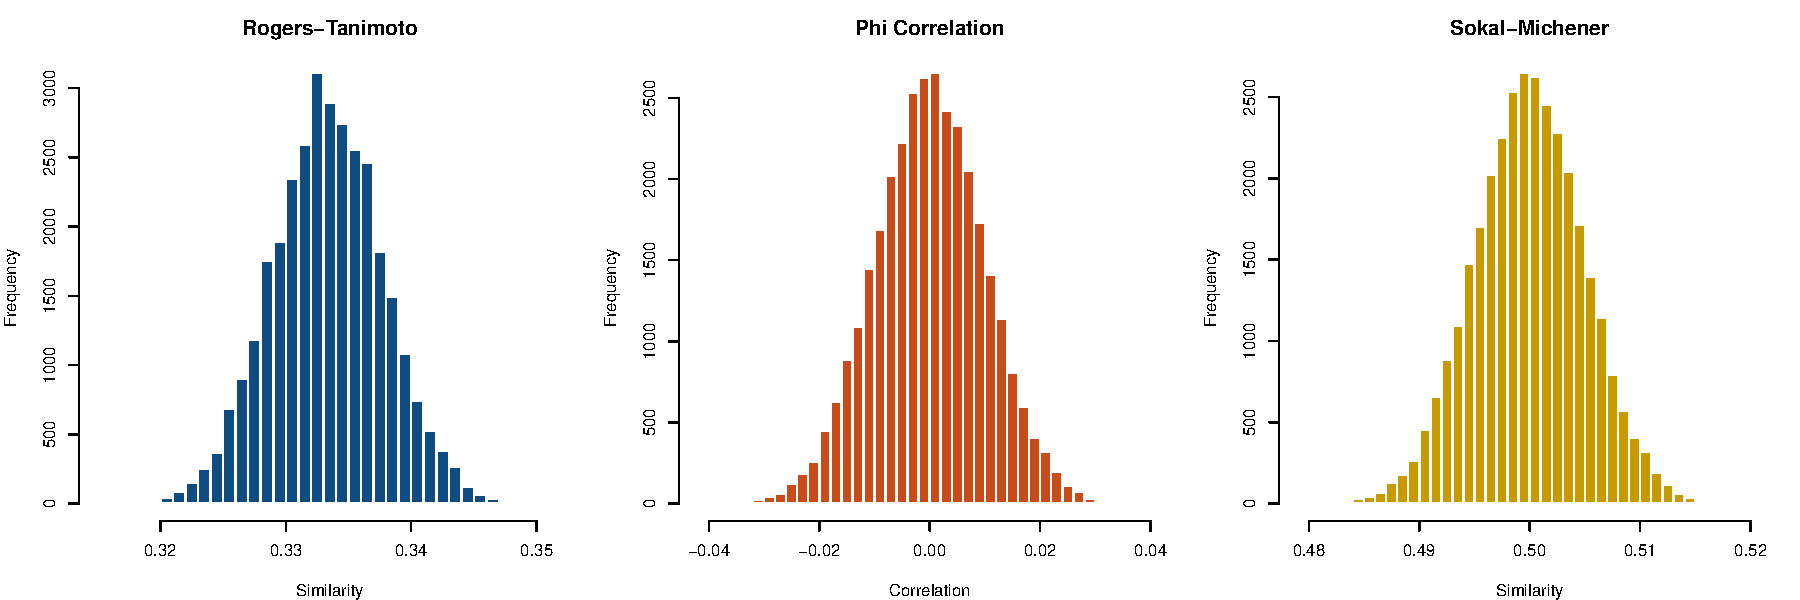
\includegraphics[width=\textwidth]{figures/pairwise_metrics.pdf}
\caption{Pairwise similarity and correlation metrics for all bit pairs in the
baseline sequential integer experiment.}
\label{fig:pairwise}
\end{figure}

The second dependence diagnostic studies whether sequential structure in the
inputs survives hashing. Figure~\ref{fig:input-corr} plots the Pearson
correlation between the input index and each bit value for the sequential
experiments. The correlations fluctuate tightly around zero with no persistent
bit-level pattern. In the present run, the largest absolute input-bit
correlation is about $0.033$, which is small relative to the scale that would
be needed to suggest a stable structural relationship between input order and
output bits.

\begin{figure}[htbp]
\centering
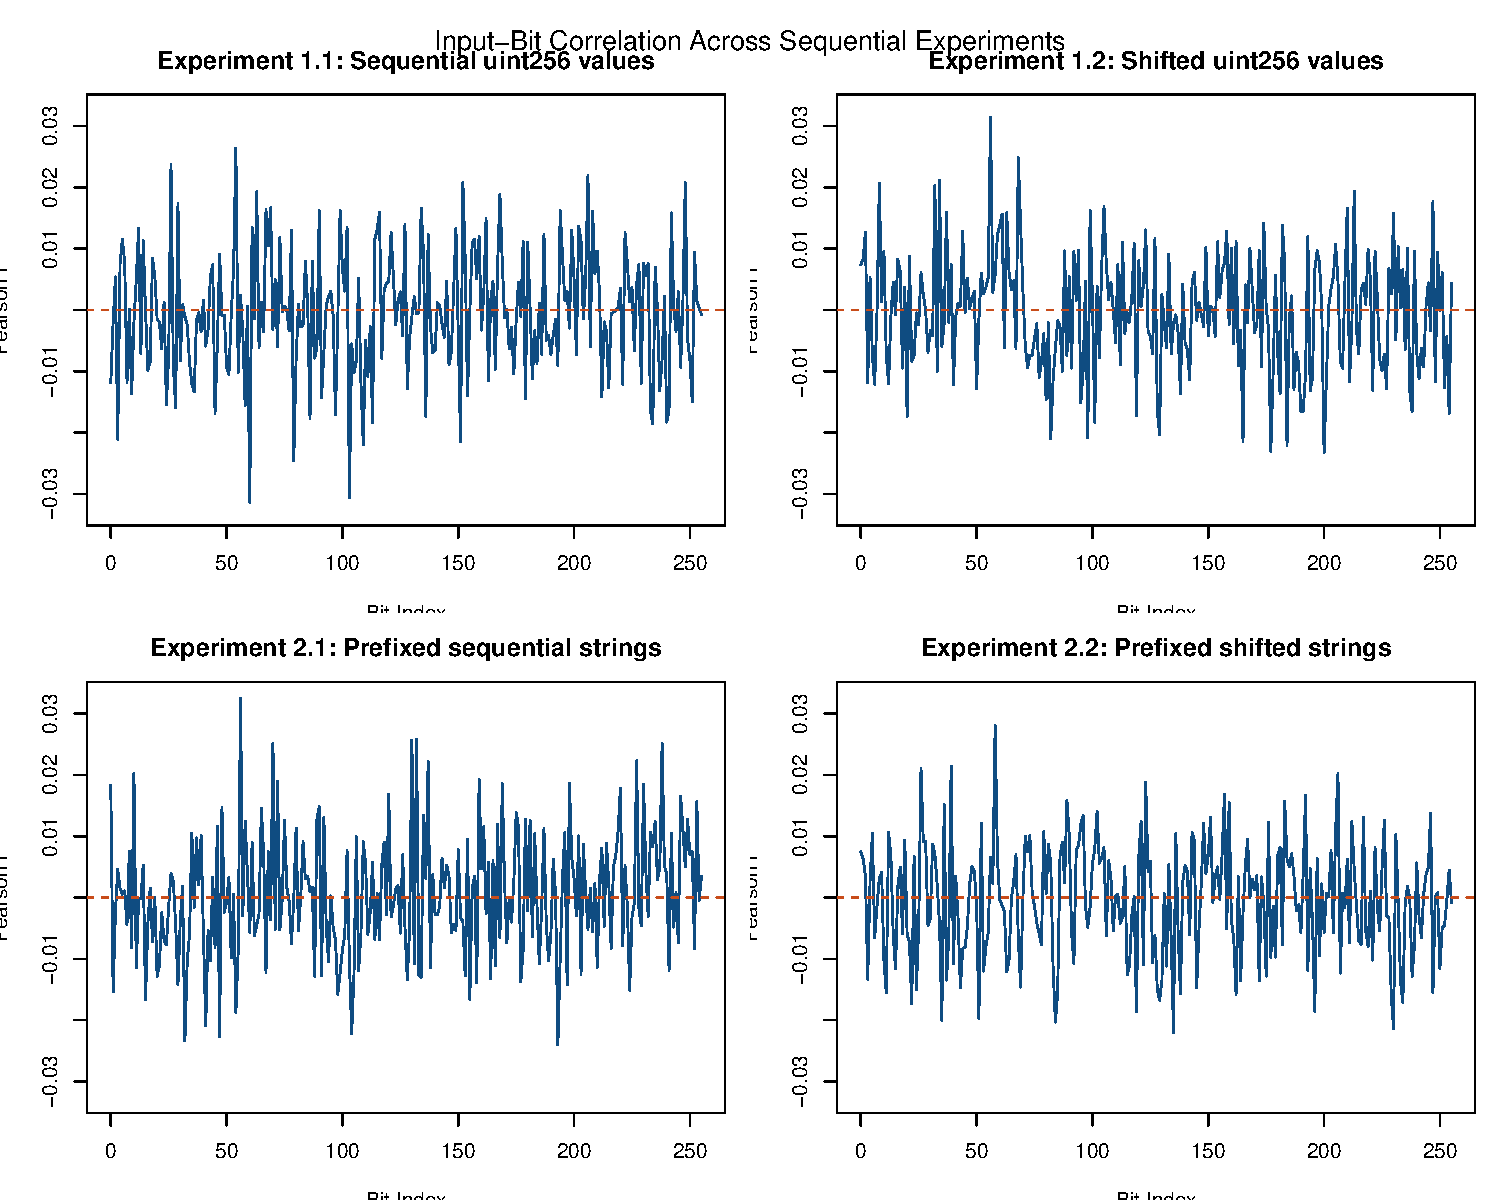
\includegraphics[width=0.92\textwidth]{figures/input_correlation_panels.pdf}
\caption{Pearson correlation between input index and each output bit for the
sequential experiments.}
\label{fig:input-corr}
\end{figure}

Finally, Figure~\ref{fig:acf} summarizes serial dependence by plotting the mean
and maximum absolute autocorrelation across the $256$ bits for lags $1$ through
$30$. These quantities remain small across the tested sequential inputs. The
largest observed maximum absolute autocorrelation in this run is below $0.044$.
That does not prove serial independence, but it does suggest that simple lag
structure is weak in the tested regimes.

\begin{figure}[htbp]
\centering
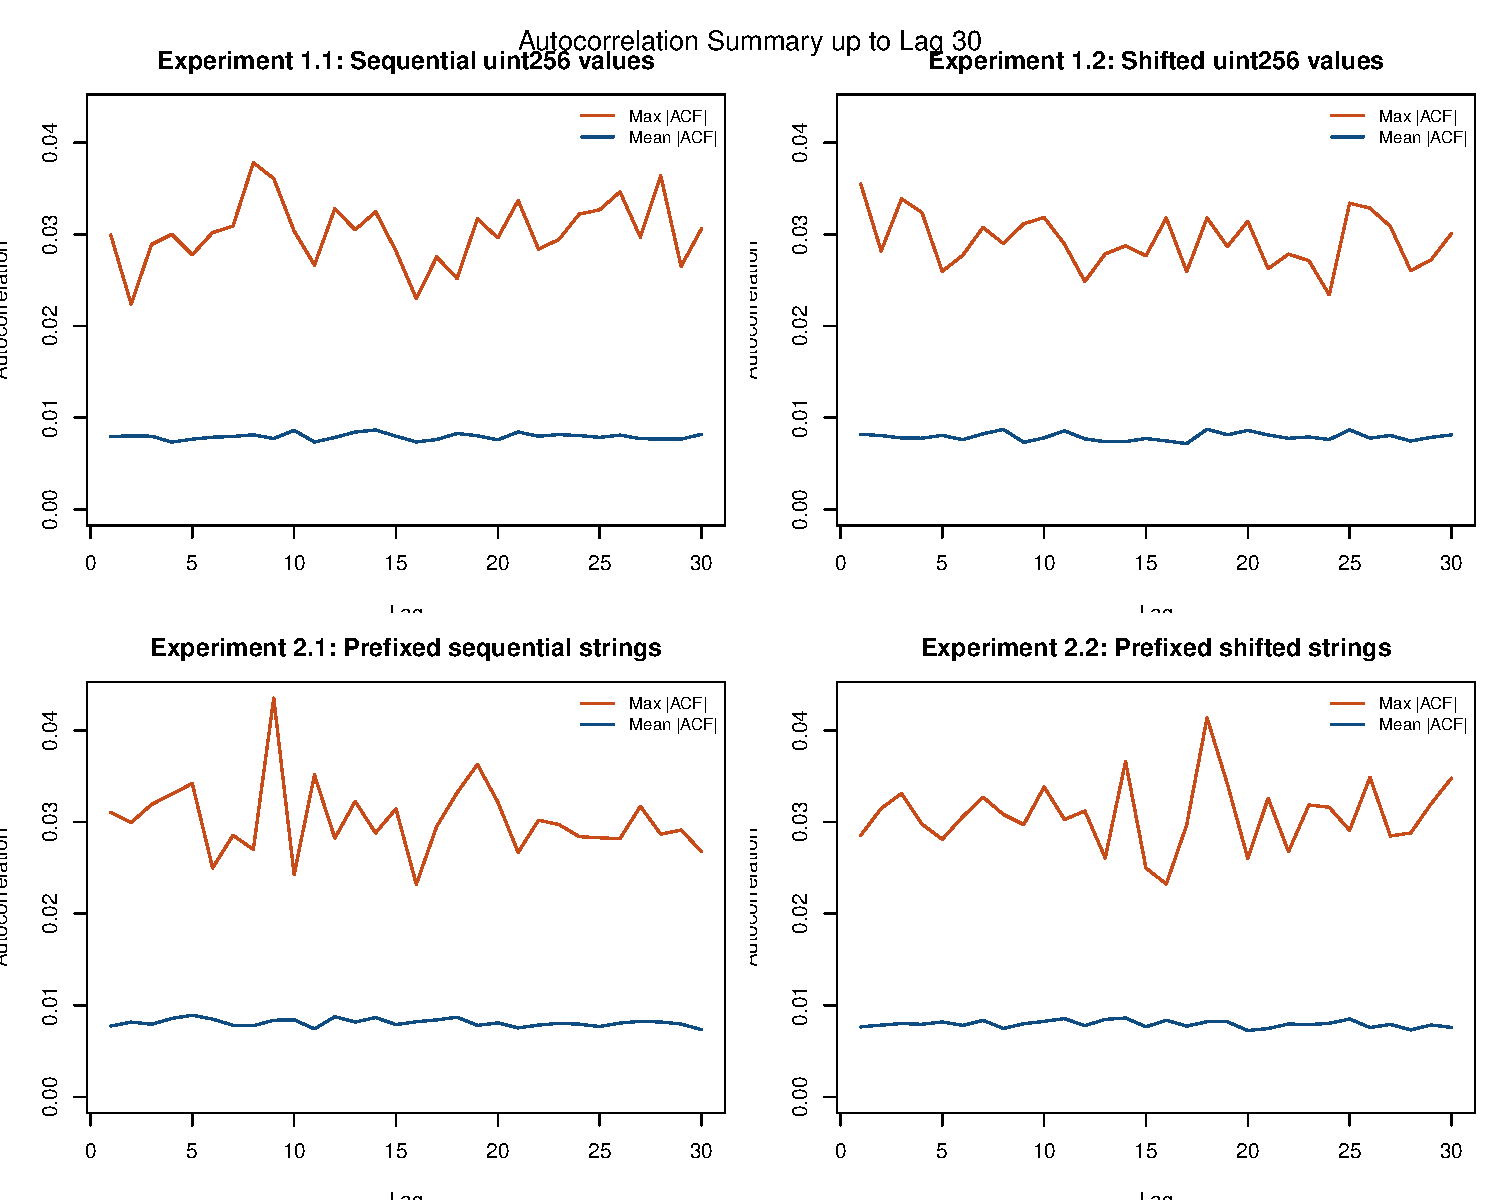
\includegraphics[width=0.92\textwidth]{figures/autocorrelation_panels.pdf}
\caption{Mean and maximum absolute bit-level autocorrelation by lag for the
sequential experiments.}
\label{fig:acf}
\end{figure}

\section{Normalization Diagnostics}

The revised theory note uses the practical normalization $(S-128)/8$, where $S$
is the count of $1$'s in a 256-bit hash. The natural numerical question is
therefore whether the empirical bit model implies values close to
\[
\hat\mu = \sum_{i=1}^{256} \hat p_i \approx 128
\qquad \text{and} \qquad
\hat\sigma = \sqrt{\sum_{i=1}^{256}\hat p_i(1-\hat p_i)} \approx 8.
\]

Figure~\ref{fig:normalization} plots the deviations $\hat\mu - 128$ and
$\hat\sigma - 8$ across the six experiment families. The deviations are small in
every case, which supports the practical scaling used in the Gaussian RNG
construction. In the present run, the largest absolute deviation in $\hat\mu$ is
about $0.171$, while the largest absolute deviation in $\hat\sigma$ is below
$0.001$. Table~\ref{tab:normalization} reports the corresponding values
explicitly.

\begin{figure}[htbp]
\centering
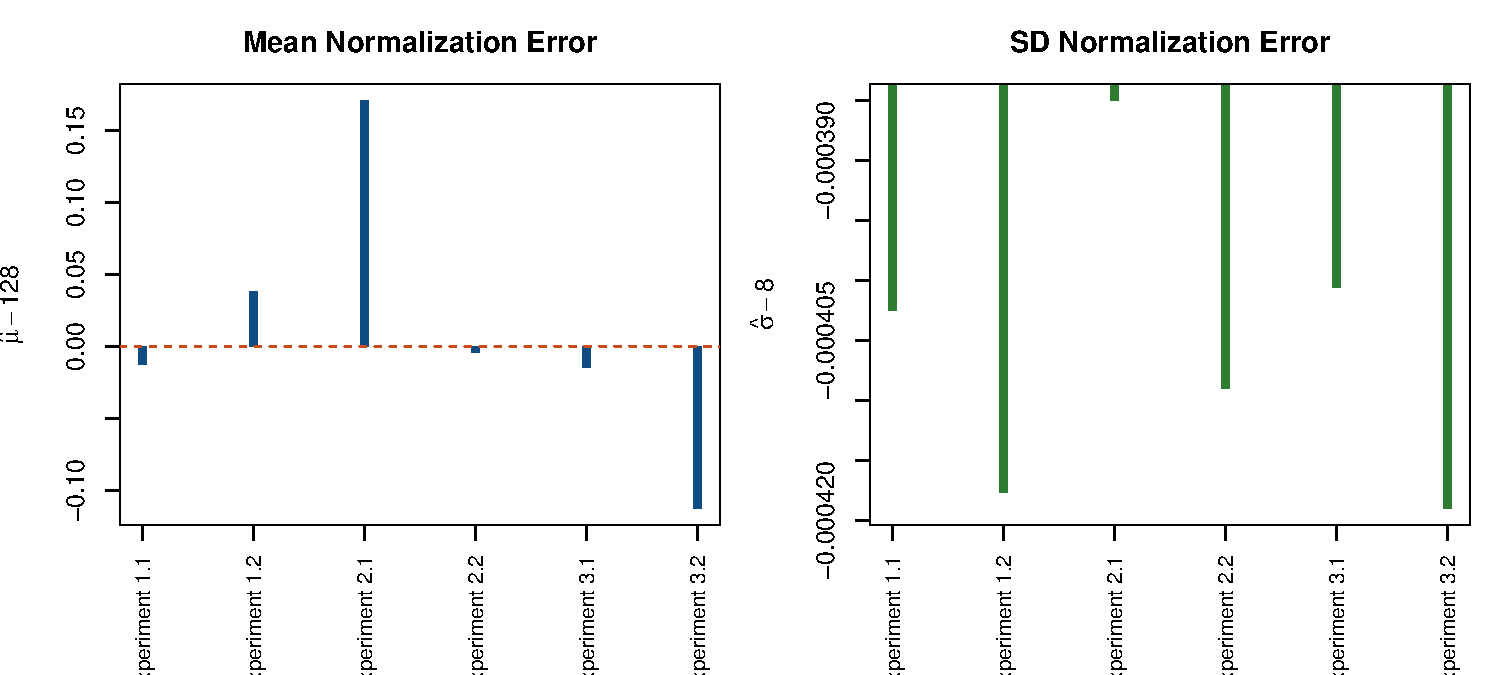
\includegraphics[width=0.92\textwidth]{figures/normalization_errors.pdf}
\caption{Empirical normalization errors relative to the practical centering and
scaling constants $128$ and $8$.}
\label{fig:normalization}
\end{figure}

\begin{table}[htbp]
\centering
\begin{tabular}{lrrrrrr}
\hline
Experiment & $\hat\mu$ & $\hat\mu-128$ & $(\hat\mu-128)/8$ & $\hat\sigma$ & $s_S$ & $s_S^2/\hat\sigma^2$ \\
\hline
Experiment 1.1 & 127.9873 & -0.0127 & -0.0016 & 7.9996 & 7.9854 & 0.9964 \\
Experiment 1.2 & 128.0384 & 0.0384 & 0.0048 & 7.9996 & 7.9520 & 0.9881 \\
Experiment 2.1 & 128.1708 & 0.1708 & 0.0213 & 7.9996 & 8.0663 & 1.0167 \\
Experiment 2.2 & 127.9960 & -0.0040 & -0.0005 & 7.9996 & 8.0182 & 1.0047 \\
Experiment 3.1 & 127.9854 & -0.0146 & -0.0018 & 7.9996 & 7.9888 & 0.9973 \\
Experiment 3.2 & 127.8874 & -0.1126 & -0.0141 & 7.9996 & 7.9731 & 0.9934 \\
\hline
\end{tabular}

\caption{Estimated centering and scaling implied by the empirical bit
probabilities.}
\label{tab:normalization}
\end{table}

\section{Popcount Distribution Diagnostics}

The next question is whether the count of $1$'s itself behaves like a Gaussian
random variable after centering and scaling. Figure~\ref{fig:cdf} compares the
empirical CDF from a representative sample of $3{,}000$ popcounts to the
Gaussian CDF with mean $128$ and standard deviation $8$. The fit is already
visually close.

\begin{figure}[htbp]
\centering
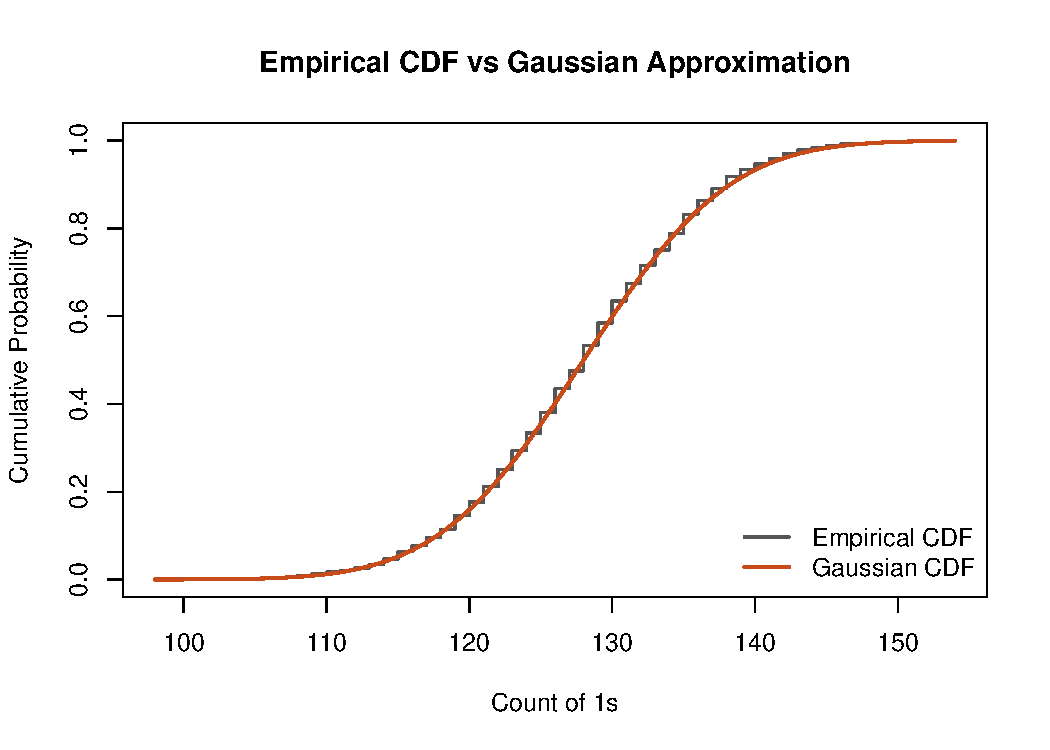
\includegraphics[width=0.78\textwidth]{figures/popcount_cdf.pdf}
\caption{Empirical CDF of the popcount against the Gaussian CDF with mean $128$
and standard deviation $8$.}
\label{fig:cdf}
\end{figure}

Figure~\ref{fig:qq} strengthens that comparison by showing QQ plots for all six
experiment families. Most of the deviation from the identity line is minor and
concentrated in the tails, which is the typical finite-sample behavior one would
expect from a discrete approximation to a continuous Gaussian law.

\begin{figure}[htbp]
\centering
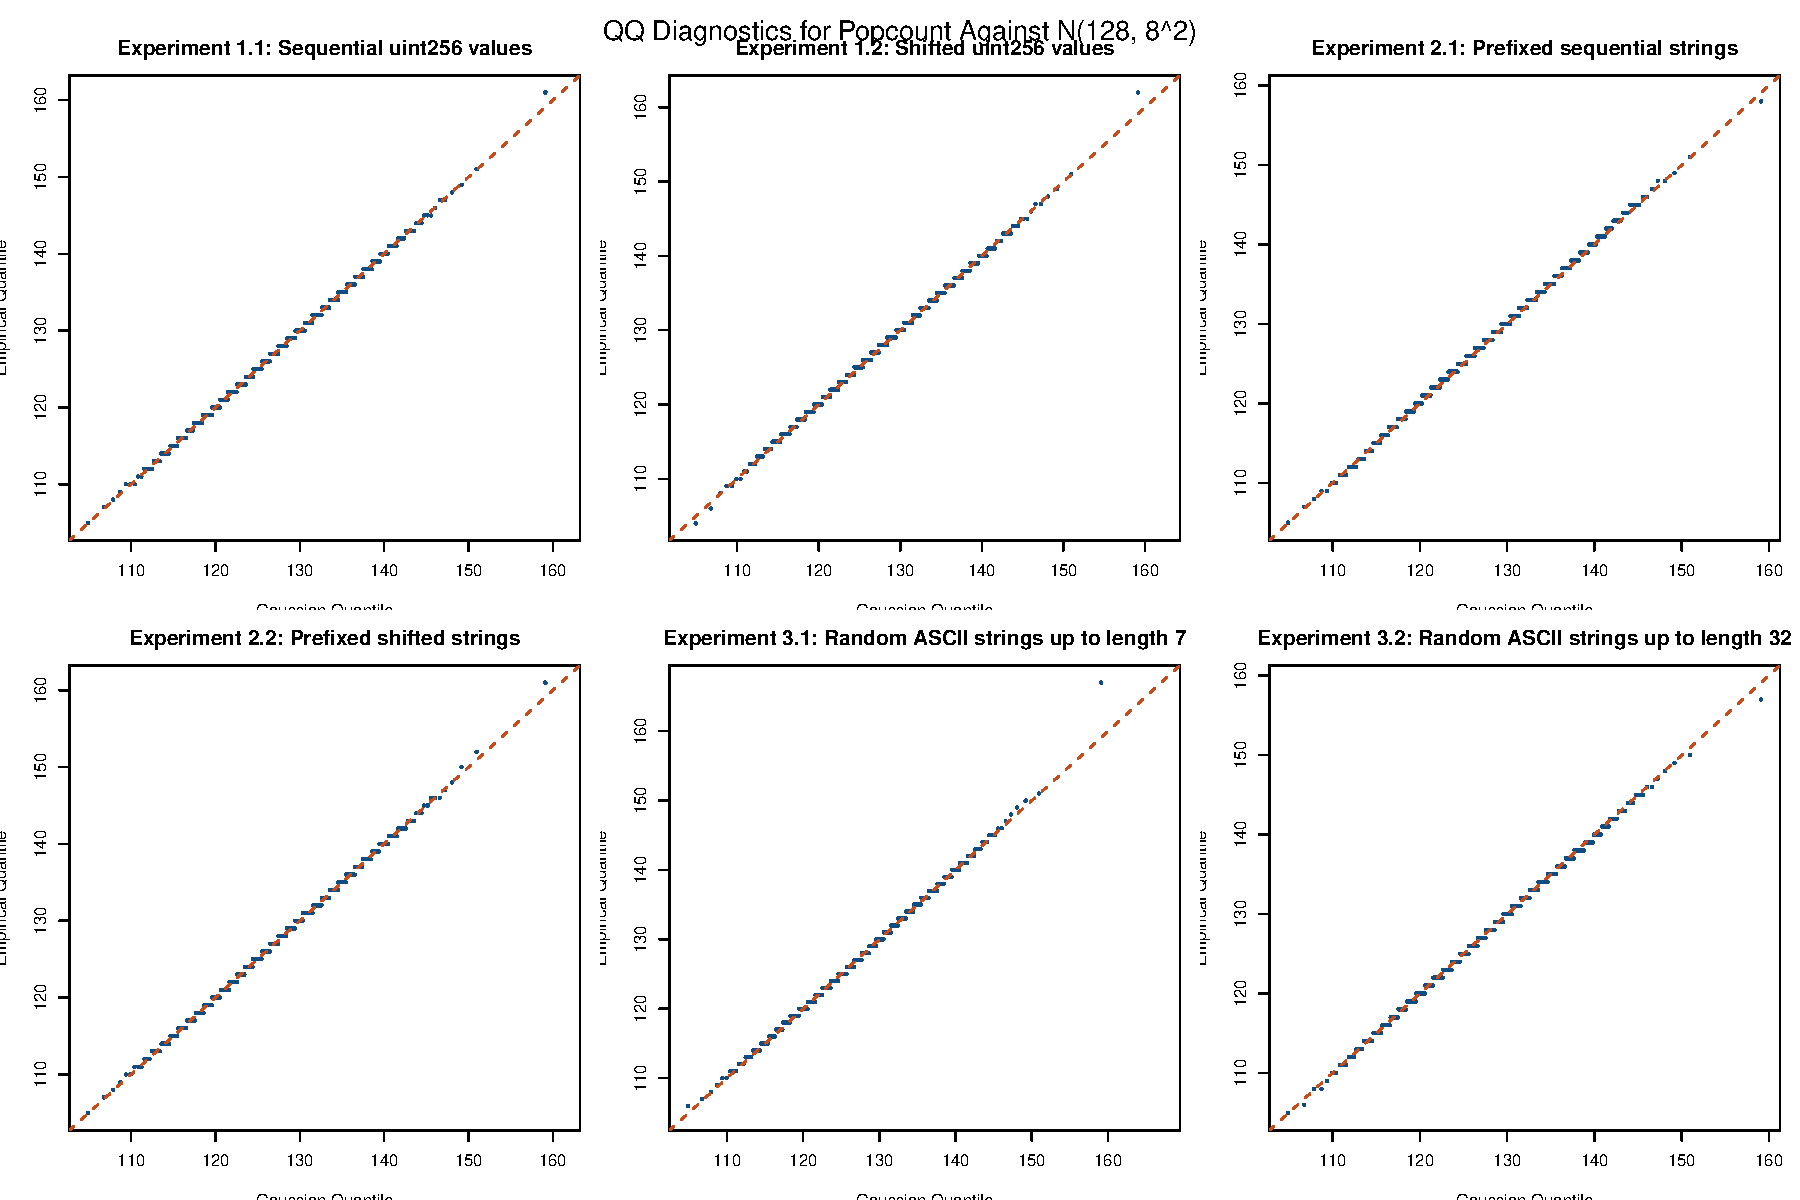
\includegraphics[width=\textwidth]{figures/popcount_qq_panels.pdf}
\caption{QQ diagnostics comparing empirical popcount quantiles to the quantiles
of $N(128, 8^2)$.}
\label{fig:qq}
\end{figure}

Figure~\ref{fig:tails} compares the empirical two-sided tail probabilities
$\mathbb{P}(|(S-128)/8| \ge z)$ to the corresponding Gaussian tail
probabilities over a range of thresholds. This gives a more direct view of
whether the practical Gaussian approximation is under- or over-estimating tail
mass in the finite 256-bit setting.

\begin{figure}[htbp]
\centering
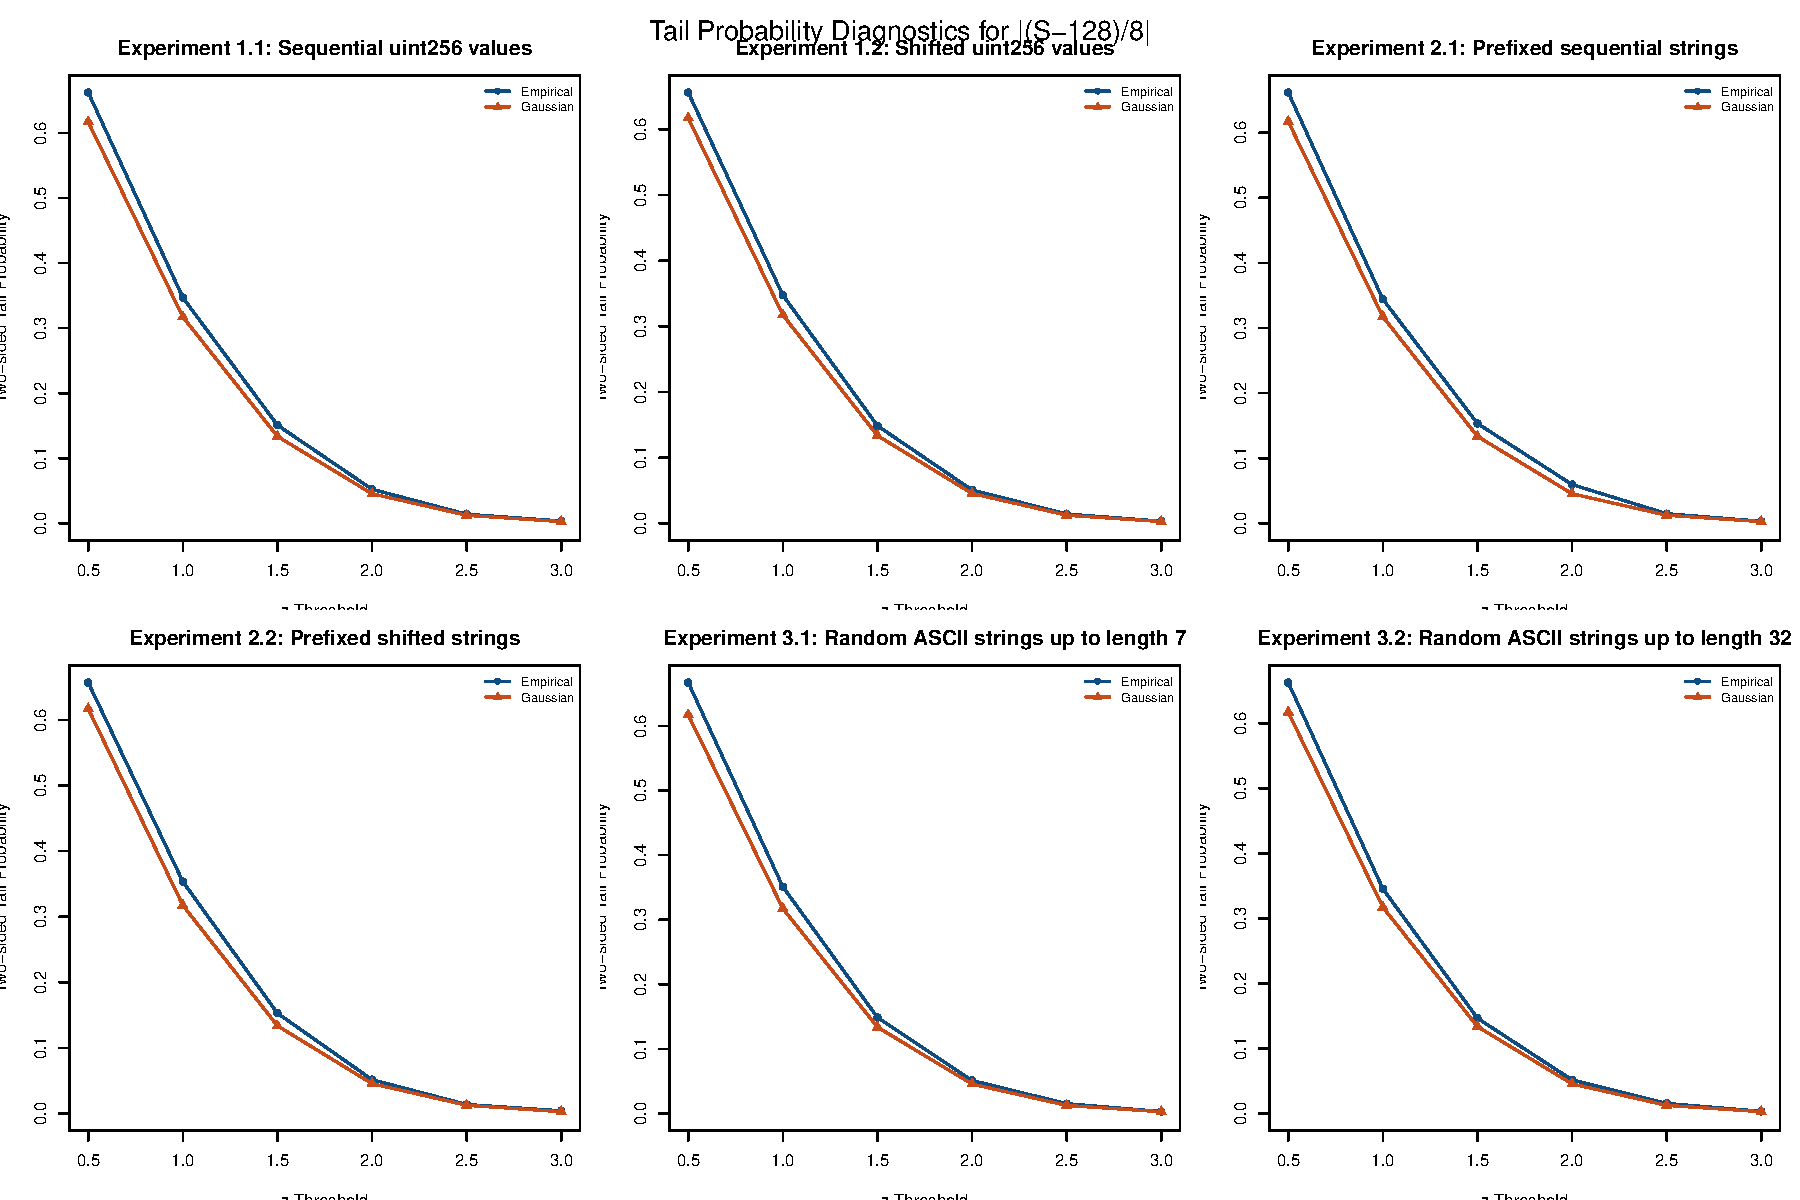
\includegraphics[width=\textwidth]{figures/popcount_tail_panels.pdf}
\caption{Empirical and Gaussian two-sided tail probabilities for the
standardized popcount.}
\label{fig:tails}
\end{figure}

Table~\ref{tab:distribution} summarizes the finite-sample Gaussian fit using the
Kolmogorov-Smirnov distance, a one-dimensional Wasserstein distance, skewness,
excess kurtosis, and the absolute two-sided tail error at $z=2$. These metrics
remain modest across all six experiment families and reinforce the claim that
the popcount is close enough to Gaussian for the intended on-chain use. In this
run, the Kolmogorov-Smirnov distance lies between roughly $0.028$ and $0.036$,
and the absolute two-sided tail error at $z=2$ lies between roughly $0.005$ and
$0.014$.

\begin{table}[htbp]
\centering
\begin{tabular}{lrrrrrrr}
\hline
Experiment & KS$_{\mathcal N}$ & KS$_{\mathrm{Bin}}$ & $W_1^{\mathcal N}$ & $W_1^{\mathrm{Bin}}$ & Skewness & Excess Kurtosis & $|\Delta T_2|$ \\
\hline
Experiment 1.1 & 0.0282 & 0.0036 & 0.2546 & 0.0490 & 0.0007 & -0.0153 & 0.0069 \\
Experiment 1.2 & 0.0311 & 0.0062 & 0.2624 & 0.0838 & -0.0273 & 0.0419 & 0.0053 \\
Experiment 2.1 & 0.0363 & 0.0117 & 0.2924 & 0.1927 & -0.0137 & 0.0437 & 0.0141 \\
Experiment 2.2 & 0.0288 & 0.0052 & 0.2591 & 0.0669 & 0.0019 & 0.0175 & 0.0060 \\
Experiment 3.1 & 0.0329 & 0.0090 & 0.2684 & 0.0972 & 0.0602 & 0.0009 & 0.0055 \\
Experiment 3.2 & 0.0302 & 0.0067 & 0.2695 & 0.1129 & -0.0235 & 0.0000 & 0.0061 \\
\hline
\end{tabular}

\caption{Finite-sample diagnostics for the Gaussian approximation to the
popcount. The column $|\Delta T_2|$ is the absolute error in the two-sided tail
probability at $z=2$.}
\label{tab:distribution}
\end{table}

\section{Sequence Diagnostics}

The previous sections study one-shot hash outputs. The actual Gaussian RNG,
however, is consumed as a sequence by repeatedly hashing the previous state. To
study that usage directly, four repeated-hash chains are generated from four
representative seeds:
\[
H_1 = \texttt{keccak256}(\text{seed}),
\qquad
H_{t+1} = \texttt{keccak256}(H_t),
\]
and the corresponding popcount sequence
\[
S_t = \text{number of 1's in } H_t
\]
is analyzed for $t = 1, \dots, 10{,}000$.

Figure~\ref{fig:seq-acf} plots the autocorrelation of the popcount sequence for
lags $1$ through $30$. Figure~\ref{fig:seq-scatter} plots $S_t$ against
$S_{t+1}$ for the same chains. These diagnostics are intended to detect visible
serial structure in the generator itself, rather than only in isolated hash
outputs. In the present run, the lag-1 correlation lies between roughly $0.001$
and $0.018$, while the maximum absolute autocorrelation up to lag $30$ remains
below roughly $0.036$ for all four chains.

\begin{figure}[htbp]
\centering
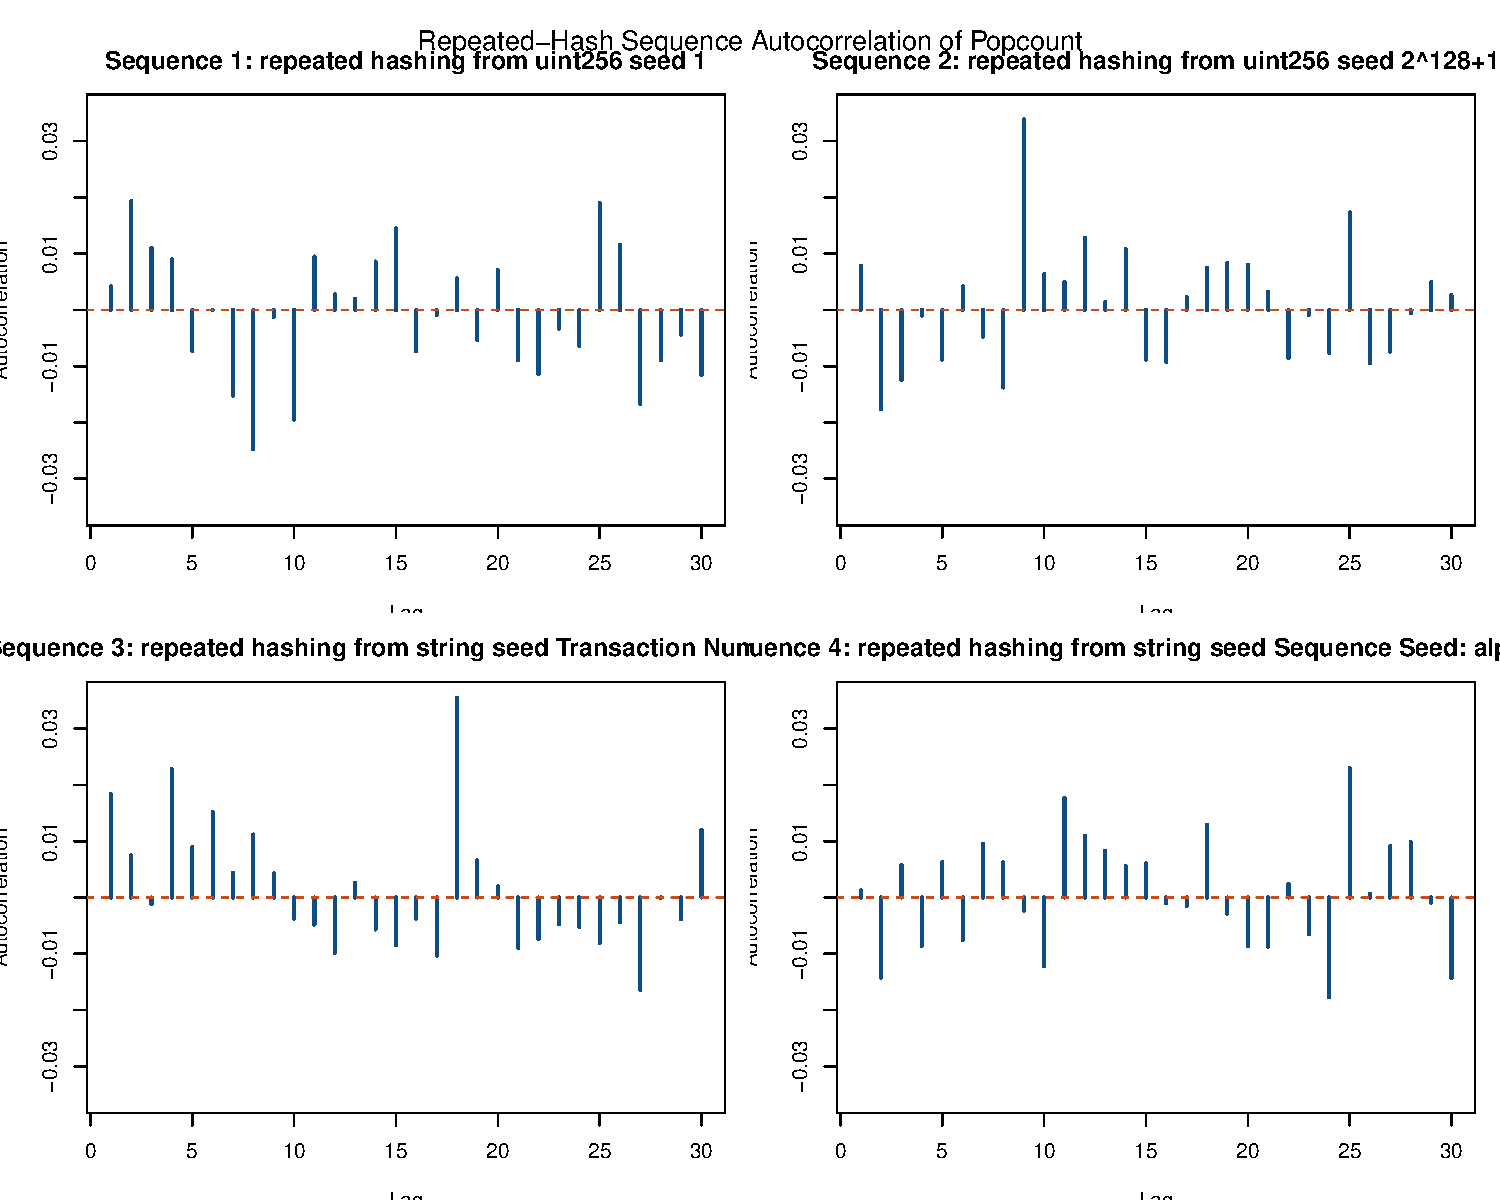
\includegraphics[width=0.92\textwidth]{figures/sequence_acf_panels.pdf}
\caption{Autocorrelation of the popcount sequence for four repeated-hash
chains.}
\label{fig:seq-acf}
\end{figure}

\begin{figure}[htbp]
\centering
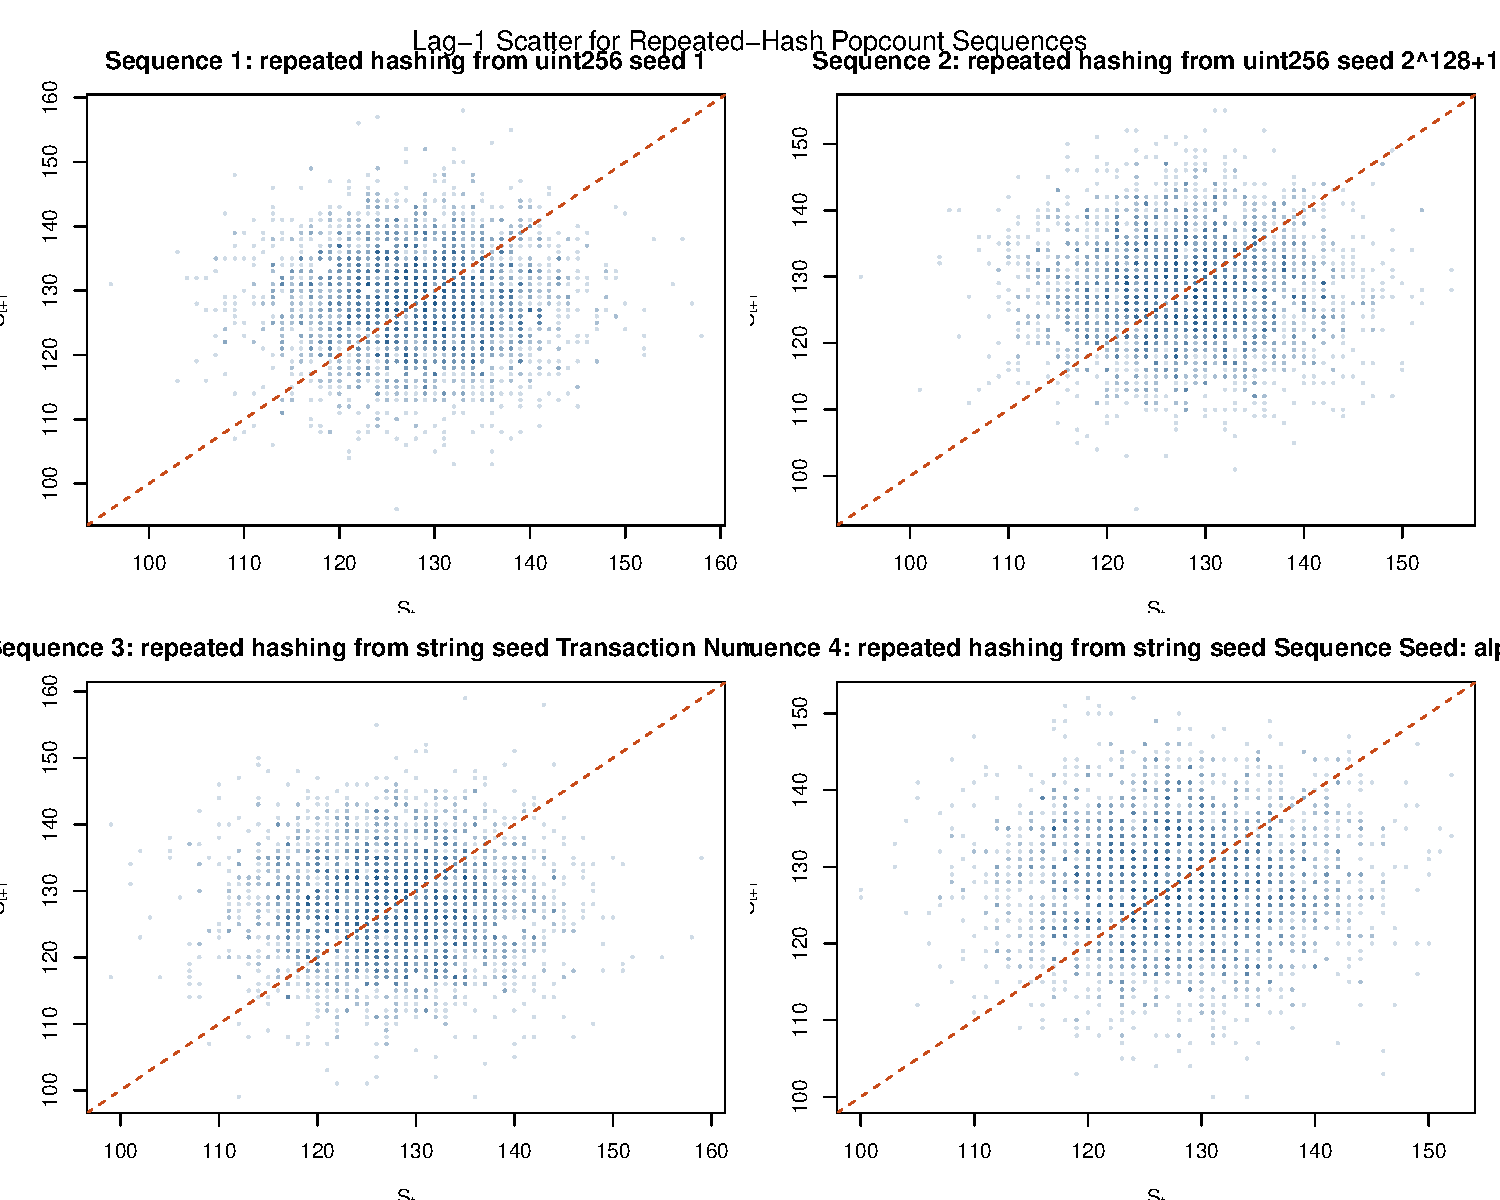
\includegraphics[width=0.92\textwidth]{figures/sequence_scatter_panels.pdf}
\caption{Lag-1 scatter plots for the popcount sequence under repeated hashing.}
\label{fig:seq-scatter}
\end{figure}

Table~\ref{tab:sequence} summarizes the same study by reporting the mean and
standard deviation of the sequence, the lag-1 correlation, and the largest
absolute autocorrelation over lags up to $30$. These are the main numerical
checks for whether the recursive generator introduces visible short-lag
dependence. The associated runs-test $z$-scores also remain modest in this run,
which is consistent with the visual impression that the repeated-hash generator
does not display an obvious short-lag pattern for the tested seeds.

\begin{table}[htbp]
\centering
\begin{tabular}{lrrrrrr}
\hline
Sequence & Mean Count & SD Count & Lag-1 Corr & Max $|\rho_h|$ & Runs $z$ & $|\Delta T_2|$ \\
\hline
Sequence 1 & 127.9579 & 7.9600 & 0.0042 & 0.0248 & 0.1287 & 0.0027 \\
Sequence 2 & 128.0153 & 7.9580 & 0.0079 & 0.0339 & -0.1537 & 0.0083 \\
Sequence 3 & 128.0109 & 7.9452 & 0.0184 & 0.0354 & -1.4950 & 0.0047 \\
Sequence 4 & 127.8900 & 7.9386 & 0.0013 & 0.0230 & 0.7849 & 0.0068 \\
\hline
\end{tabular}

\caption{Summary diagnostics for repeated-hash popcount sequences.}
\label{tab:sequence}
\end{table}

\section{Summary Metrics}

Table~\ref{tab:summary} collects the main diagnostics for the six experiments.
The maximum absolute bit bias, mean and standard deviation of the count of $1$'s
in each 256-bit hash, and the strongest observed input-correlation and
autocorrelation diagnostics are all compatible with the working model used in
the Gaussian random number generator paper. In particular, the empirical mean of
the count of $1$'s remains close to $128$ and the empirical standard deviation
remains close to $8$ in every experiment, which is exactly the practical scale
used in the revised theory note.

\begin{table}[htbp]
\centering
\begin{tabular}{lrrrrr}
\hline
Experiment & Max $|\hat p_i-0.5|$ & Mean Count & SD Count & Max $|r|$ & Max $|\rho_h|$ \\
\hline
Experiment 1.1 & 0.0192 & 127.9873 & 7.9854 & 0.0314 & 0.0378 \\
Experiment 1.2 & 0.0164 & 128.0384 & 7.9520 & 0.0314 & 0.0355 \\
Experiment 2.1 & 0.0179 & 128.1708 & 8.0663 & 0.0325 & 0.0435 \\
Experiment 2.2 & 0.0166 & 127.9960 & 8.0182 & 0.0281 & 0.0414 \\
Experiment 3.1 & 0.0144 & 127.9854 & 7.9888 & -- & -- \\
Experiment 3.2 & 0.0171 & 127.8874 & 7.9731 & -- & -- \\
\hline
\end{tabular}

\caption{Summary diagnostics across all experiments. The columns ``Max
$|r|$'' and ``Max $|\rho_h|$'' are only applicable to the sequential
experiments.}
\label{tab:summary}
\end{table}

\section{Limitations}

This study has three important limitations.

\begin{enumerate}
\item The experiments cover several representative input families, not the full
input space of \texttt{keccak256}.
\item The dependence diagnostics are mainly marginal, pairwise, and low-lag
time-series checks. They do not establish full joint independence of all bits or
all forms of long-range dependence in the repeated-hash generator.
\item The study is empirical and finite-sample. It supports a practical model
for the Gaussian RNG construction, but it is not a cryptographic proof about the
hash function.
\end{enumerate}

\section{Conclusion}

The numerical evidence does not prove independence or exact fairness of the
\texttt{keccak256} bits. It does, however, support a practical working model in
which the output digits are treated as approximately independent Bernoulli
variables with success probabilities close to $0.5$. That is the empirical
assumption used by the revised Gaussian random number generator theory note.

The right way to read the study is therefore modestly: it does not certify the
model, but it does make the model harder to dismiss. For the quantities that the
Gaussian RNG actually uses, namely the count of $1$'s and its centering and
scaling, the observed behavior in these experiments is close to what the theory
requires. In particular, the empirical normalization implied by the bit
probabilities stays close to $(128, 8)$, and the popcount itself remains close
to a Gaussian benchmark under several complementary diagnostics. The repeated
hash sequence study also provides direct evidence that the recursive generator
does not exhibit obvious short-lag structure for the tested seeds.

\end{document}
